\documentclass[11pt]{article}

\usepackage[margin=2.5cm]{geometry}
\usepackage{graphicx}
\usepackage{listings}
\usepackage{xcolor}
\usepackage{hyperref}
\usepackage{parskip}

\lstset{
  basicstyle=\ttfamily\small,
  breaklines=true,
  frame=single,
  backgroundcolor=\color{gray!10},
  xleftmargin=1em,
  xrightmargin=1em
}

\title{DVA489 --- Assignment 3 \\ Attack Report: Cross-Site Request Forgery (CSRF)}
\author{Nasif Sarwar}
\date{\today}

\begin{document}
\maketitle

\section{Overview}
Squeak!'s \texttt{squeak-session} cookie is attached automatically by the
browser to every request sent to \texttt{localhost:8000}, regardless of
which page triggered the request. The unpatched application performs no
check that a request was actually intentional: it only checks that a valid
session cookie is present. This means any page the victim's browser visits
--- on any origin --- can make the victim's browser submit a squeak on
their behalf, simply by auto-submitting a hidden HTML form. The Same-Origin
Policy stops the attacker's page from \emph{reading} Squeak!'s response, but
it does nothing to stop the browser from \emph{sending} the request with
the victim's cookie attached.

\section{Task 1: Forging a request}
An attack page was built and hosted on a different origin
(\texttt{http://localhost:5500}, served separately from the Squeak!
application itself):
\begin{lstlisting}[language=HTML]
<body onload="document.forms[0].submit()">
  <h1>Get The iPhone X FREE!</h1>
  <form action="https://localhost:8000/squeak" method="POST"
        style="display:none;">
    <input type="hidden" name="squeak"
      value="Click here to get the iPhone X FREE! http://localhost:5500/">
  </form>
</body>
\end{lstlisting}
The page auto-submits the instant it loads --- no click required. While
signed in to Squeak! in the same browser, visiting this page caused a
squeak to be posted under the victim's own name without any interaction
with Squeak! itself.

\begin{figure}[h]
  \centering
  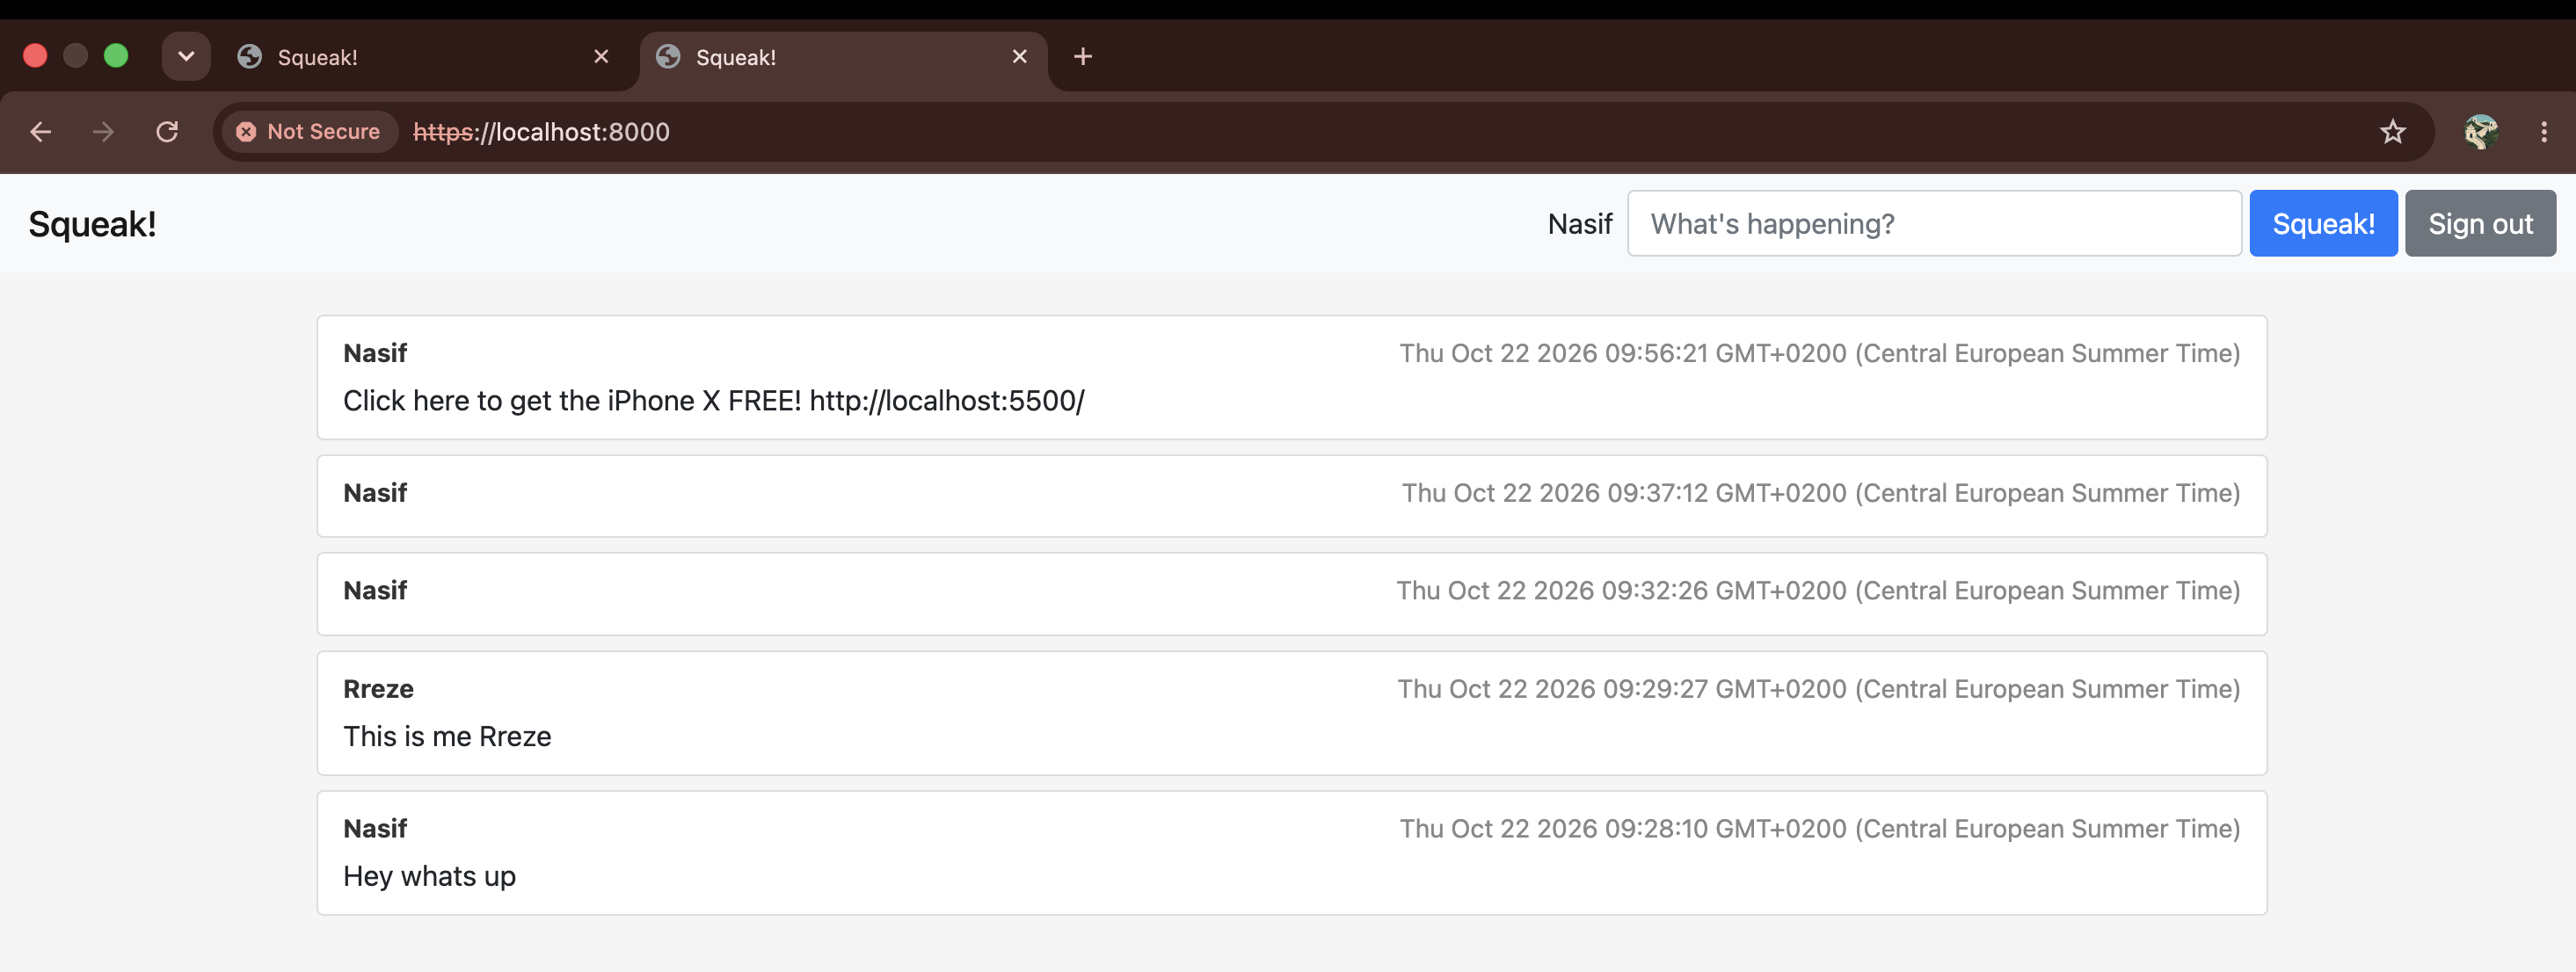
\includegraphics[width=0.9\textwidth]{images/task1-forged-squeak.png}
  \caption{A squeak posted entirely by the attacker's page, appearing under
  the victim's own name in their feed.}
\end{figure}

\section{Defense: synchronizer token pattern}
A per-session CSRF token is generated alongside the session itself and
required on every state-changing request:
\begin{lstlisting}[language=JavaScript]
function createSession(username) {
  const sessionid = crypto.randomBytes(32).toString('hex');
  sessions[sessionid] = username;
  csrfTokens[sessionid] = crypto.randomBytes(32).toString('hex');
  return sessionid;
}

function validCsrfToken(req) {
  if (!req.session) return false;
  const expected = csrfTokens[req.session.sessionid];
  return expected && req.body && req.body.csrf_token === expected;
}
\end{lstlisting}
The token is embedded in a hidden form field on the squeak form:
\begin{lstlisting}[language=HTML]
<form id="squeak-form" action="/squeak" method="POST">
  <input type="hidden" name="csrf_token" value="{{csrfToken}}">
  ...
\end{lstlisting}
A cross-origin attacker page cannot read this value: the Same-Origin Policy
blocks it from fetching and reading Squeak!'s HTML, so it has no way to
discover the current token and include it in a forged request.

\subsection{Which endpoints need the token?}
\begin{itemize}
  \item \textbf{\texttt{/squeak}} --- protected. This is the primary target
  of the attack demonstrated above, and the endpoint explicitly called out
  in the assignment.
  \item \textbf{\texttt{/signout}} --- protected. Although lower severity
  than forging a post, a plain auto-submitting form with no body at all can
  still successfully hit \texttt{/signout} and force-log-out a victim, so it
  receives the same token check.
  \item \textbf{\texttt{/signin} and \texttt{/signup}} --- \emph{not}
  token-protected, and this is a deliberate choice rather than an
  oversight. Both endpoints only accept a JSON body
  (\texttt{express.json()}). A classic CSRF relies on an auto-submitting
  HTML \texttt{<form>}, whose \texttt{enctype} can only be
  \texttt{application/x-www-form-urlencoded}, \texttt{multipart/form-data},
  or \texttt{text/plain} --- never \texttt{application/json}. A forged form
  therefore cannot produce a body that \texttt{express.json()} will parse,
  so \texttt{username}/\texttt{password} come back \texttt{undefined} and
  the request fails harmlessly. A JavaScript-based cross-origin
  \texttt{fetch} with a JSON body is theoretically possible, but that
  triggers a CORS preflight request, which the browser blocks unless the
  server responds with an \texttt{Access-Control-Allow-Origin} header ---
  something Squeak! never sends. Both endpoints are therefore already safe
  against CSRF by construction, without needing a token.
\end{itemize}

\section{Verification}
The exact same attack page from Task 1 was pointed at the patched
application. The forged request was rejected with HTTP 403, and no squeak
was posted.

\begin{figure}[h]
  \centering
  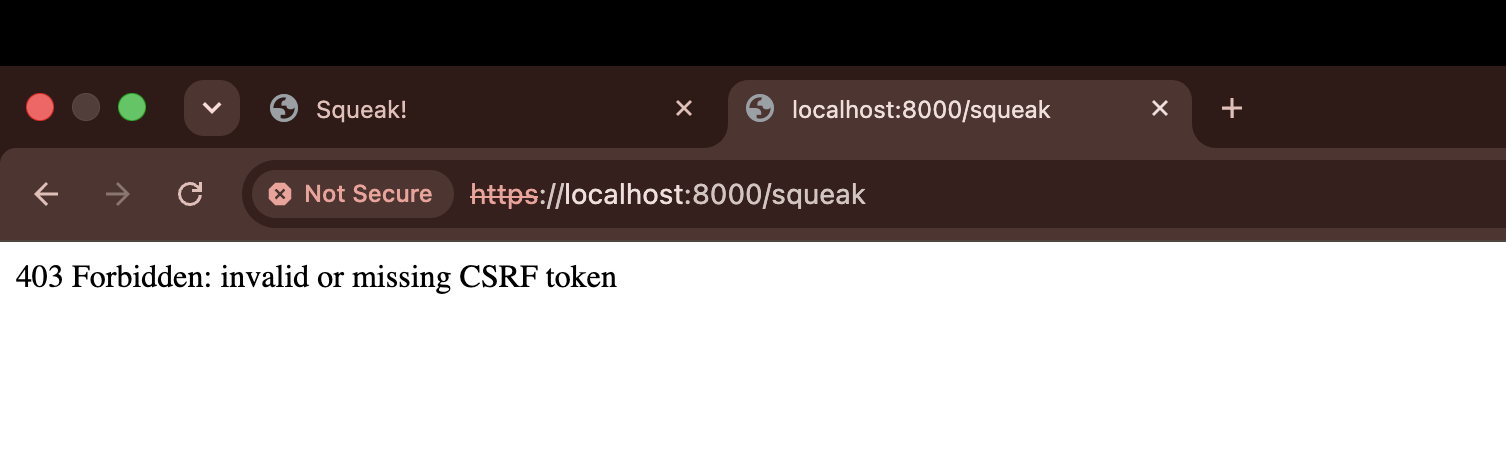
\includegraphics[width=0.8\textwidth]{images/patched-403-blocked.png}
  \caption{The patched server rejects the forged request with
  \texttt{403 Forbidden: invalid or missing CSRF token}.}
\end{figure}

\section{Conclusion}
The CSRF vulnerability let any website silently post content as any
currently-logged-in Squeak! user, exploiting the fact that cookies are
attached automatically regardless of which page initiated the request. A
synchronizer token tied to the session and unreadable by a cross-origin
page closes the gap by forcing every genuine request to prove it originated
from Squeak!'s own page, not just from a browser holding a valid cookie.

\end{document}
